\appendix
\chapter[SUPP. FIGURES]{SUPPLEMENTARY FIGURES}
\thumbtab{Appendix}{7}
\localtableofcontents
\thispagestyle{plain}
\cleardoublepage


\section{DIAGRAMS}

\subsection{COCKPIT OVERVIEW}
\begin{figure}[h]
    \centering
    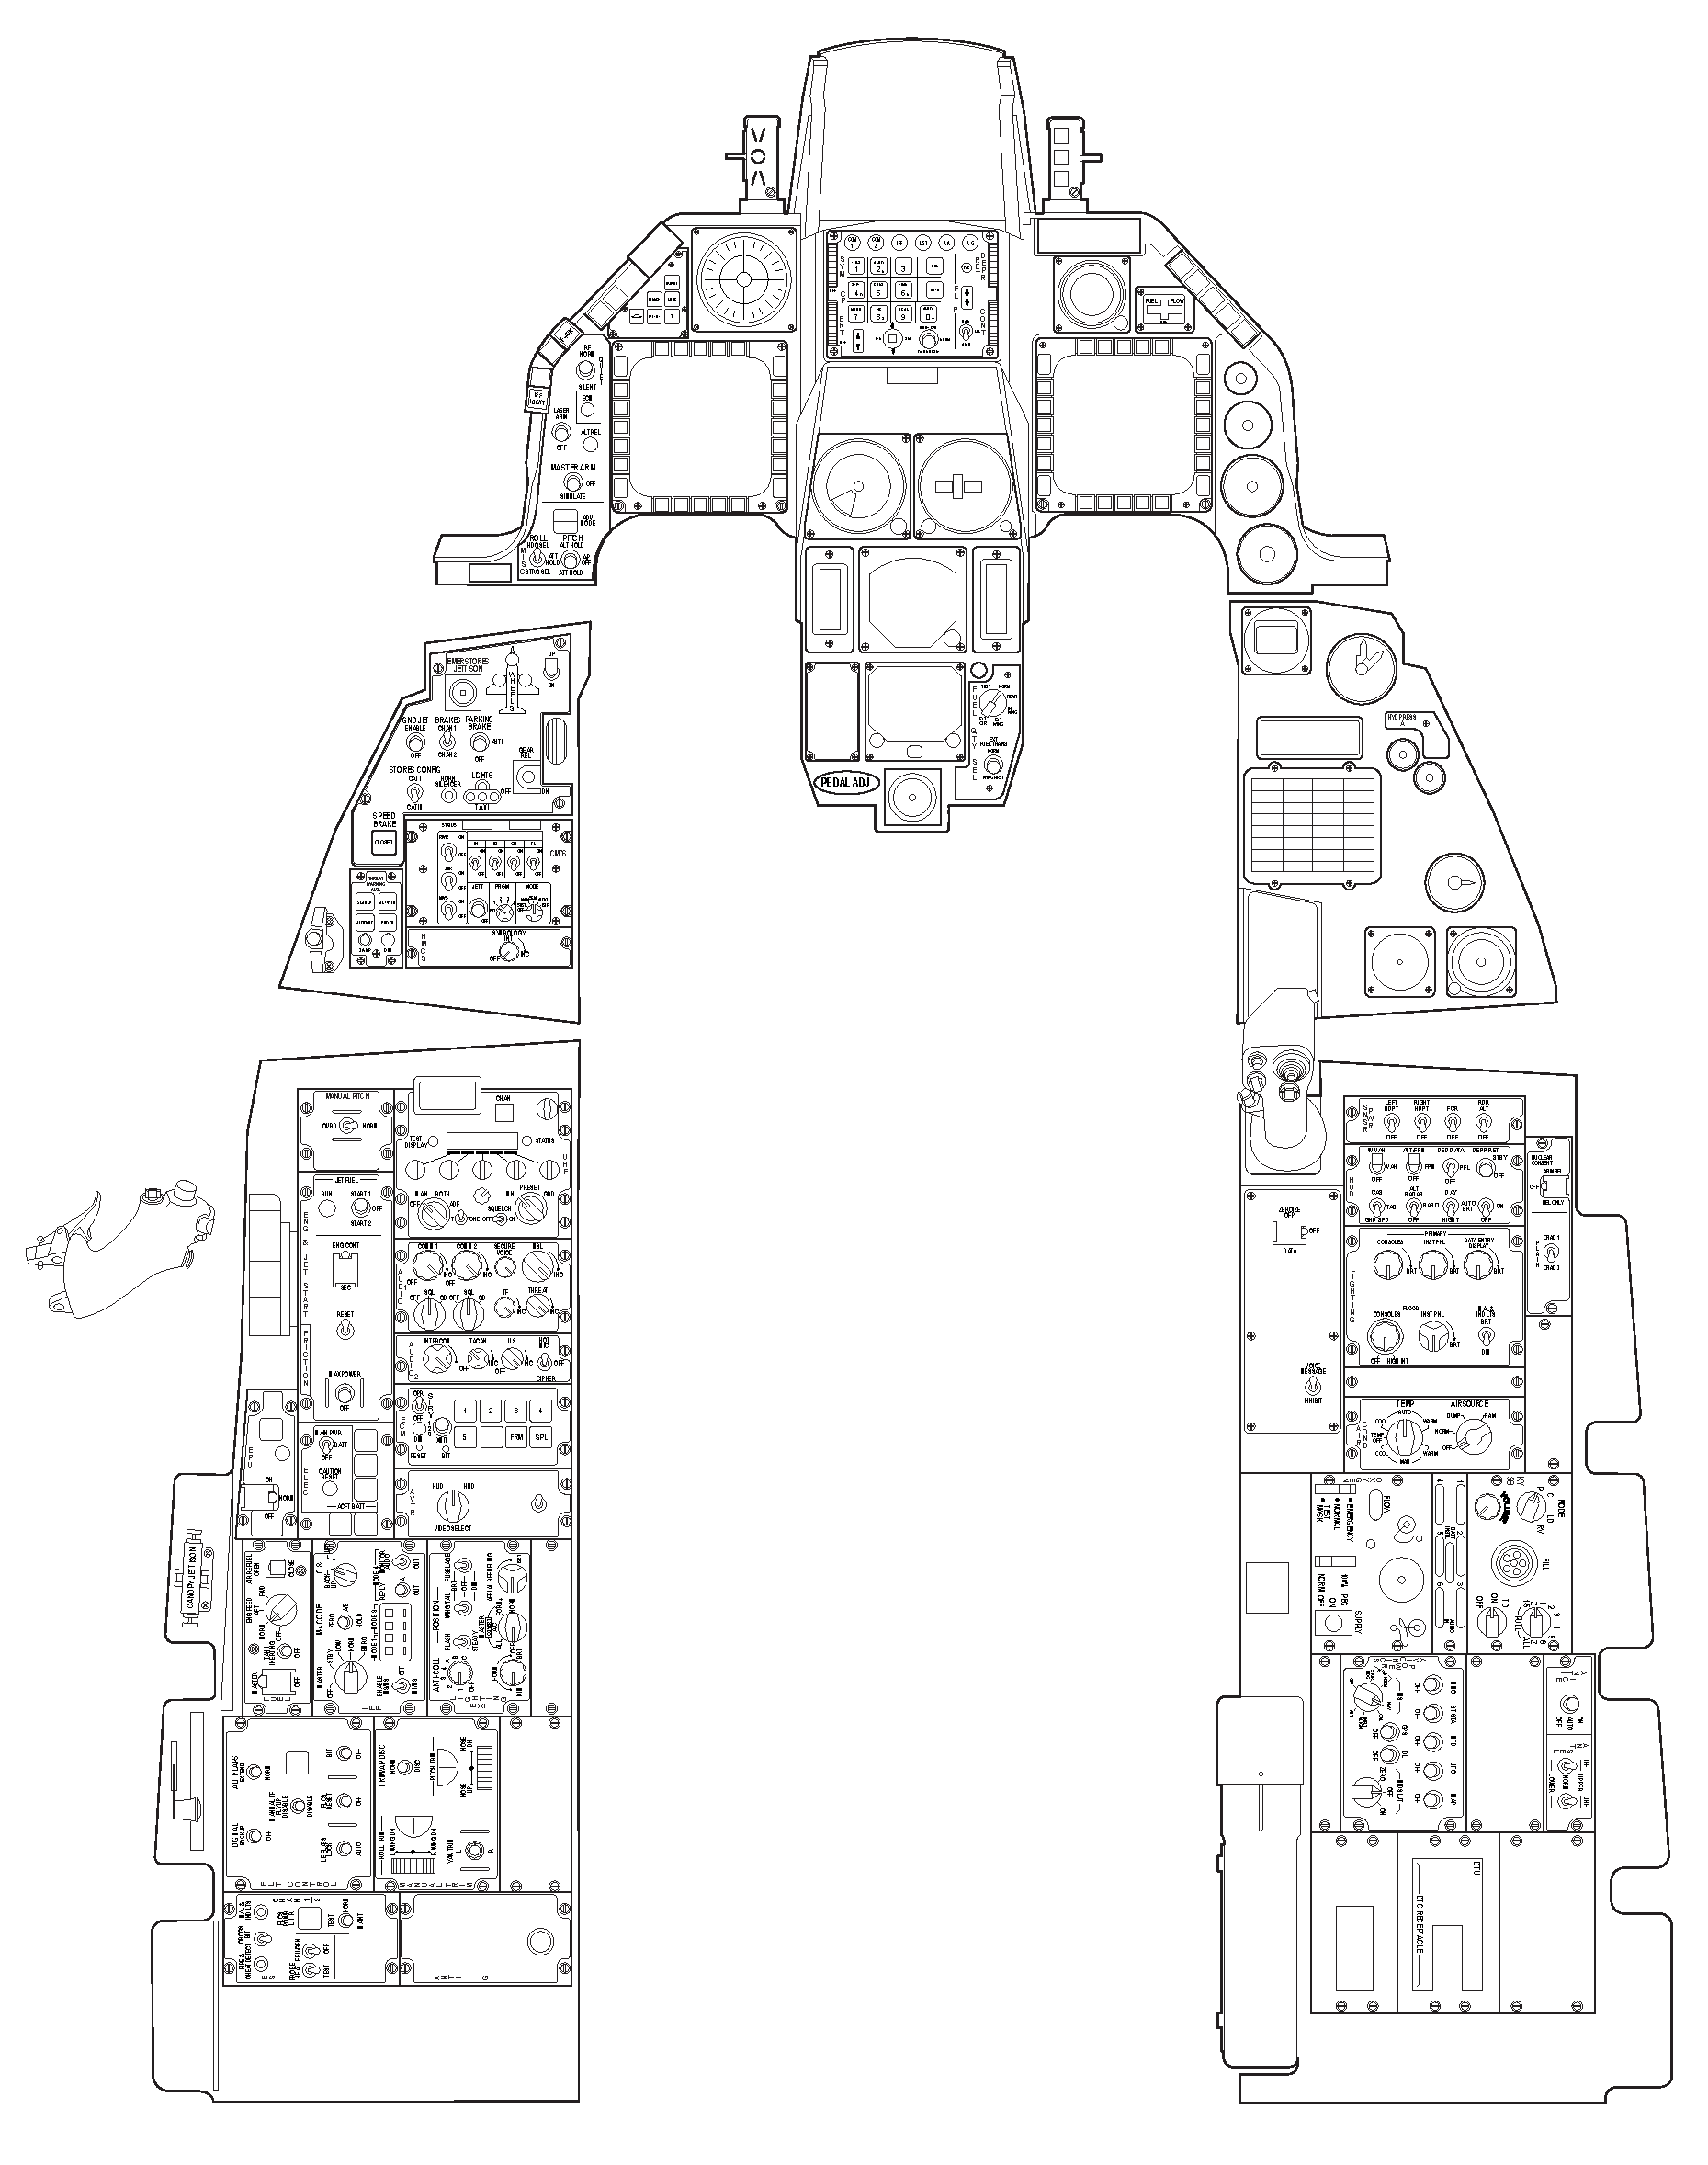
\includegraphics[
        height = 0.70\textheight,
        page = {1},
        % trim = {1.5cm, 2.5cm, 15.5cm, 1.5cm},
        % clip
    ]{diagrams/cockpit/cockpit_full.pdf}
    \caption{F-16C Block 52 Cockpit Overview}
    \label{fig:cockpitoverview}
\end{figure}

\clearpage

\subsection{FORMATION REFERENCE}

\begin{figure}[h]
    \centering
    \begin{subfigure}{0.45\linewidth}
        \centering
        \begin{tikzpicture}[auto, node distance=10mm, x=1mm, y=1mm, very thick, line cap=round,
            >={Latex[round]}
            ]
            
            \coordinate (lead) at (0,0);
            \coordinate (wing) at (30,-4);
    
            \node[yshift=-2mm] (leadfig) at (lead) {
                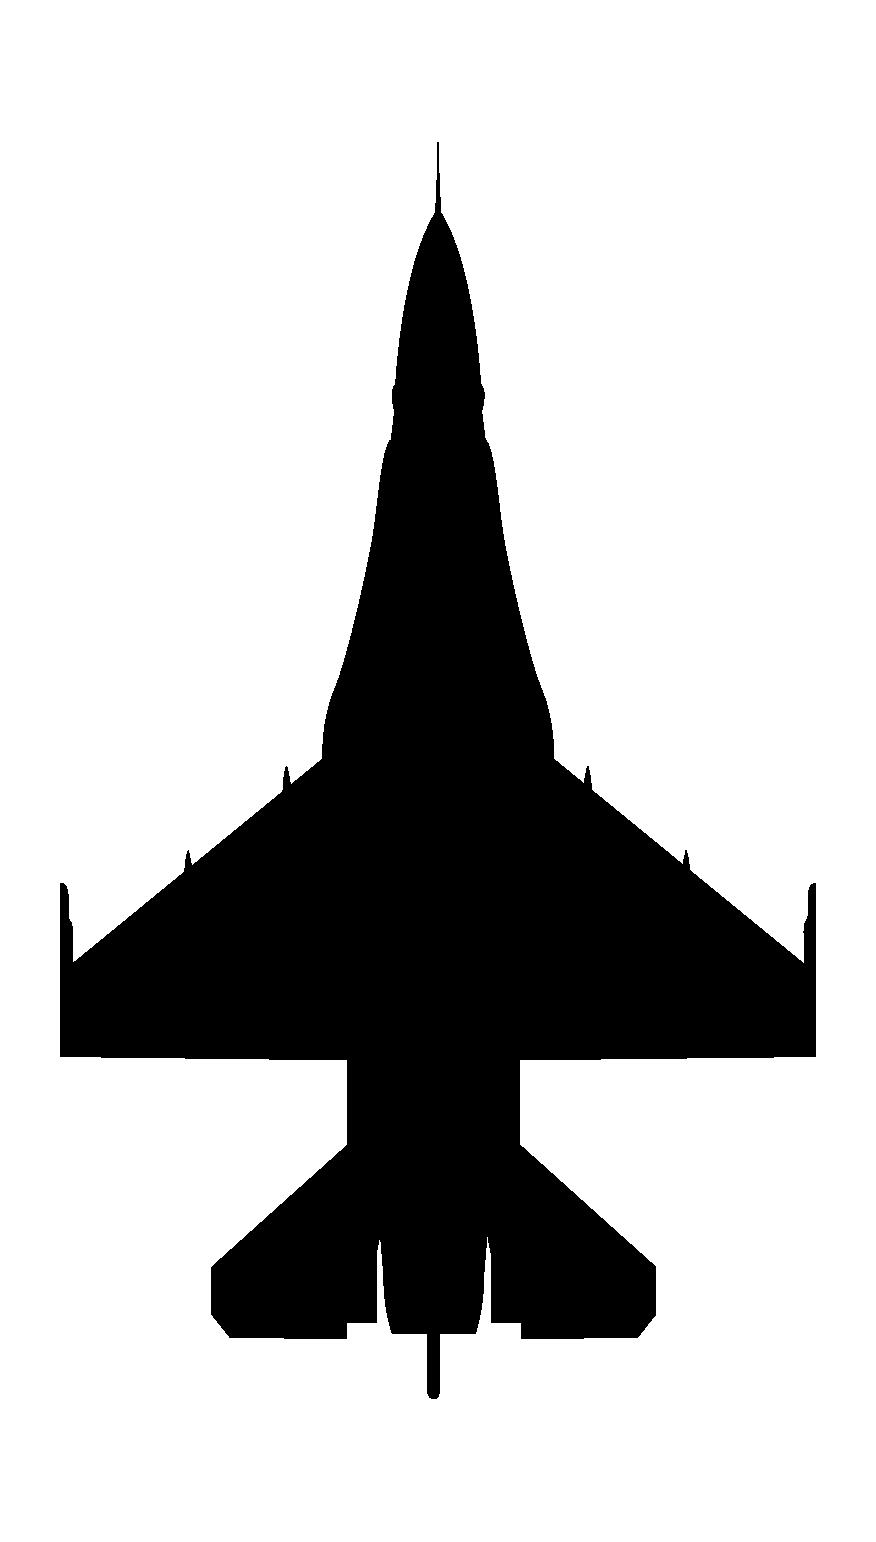
\includegraphics[
                    width=7.5mm,
                ]{diagrams/aircraft/silhouette_f16_top.pdf}
            };
            
            \node[yshift=-2mm] (wingfig) at (wing) {
                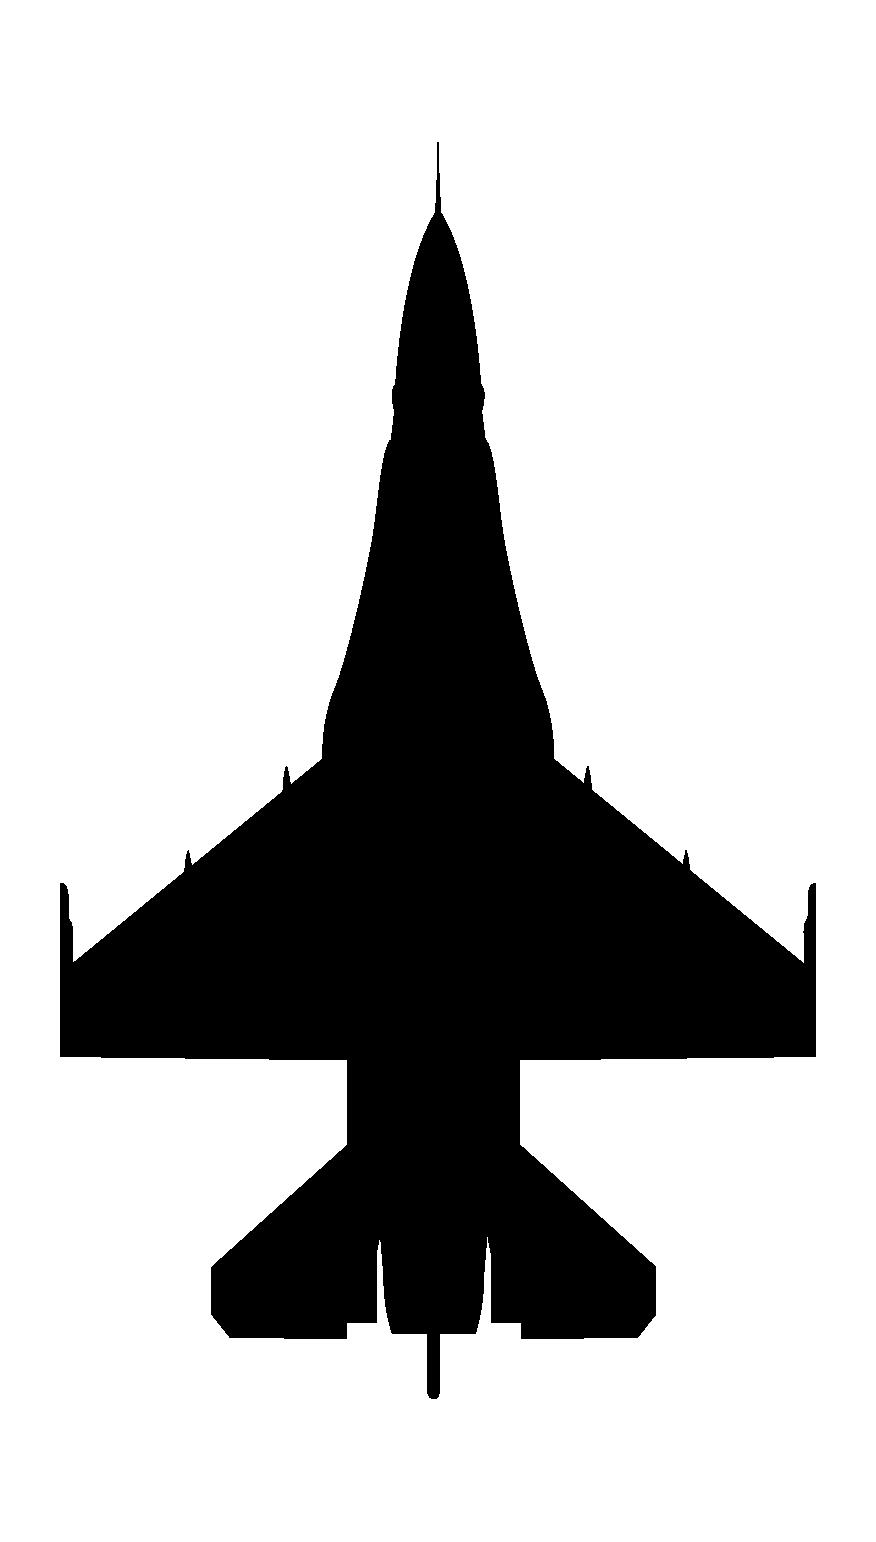
\includegraphics[
                    width=7.5mm,
                ]{diagrams/aircraft/silhouette_f16_top.pdf}
            };
    
            \draw[dotted]
            (lead) 
            -- node [font=\footnotesize] {6000'} ++(30, 0) 
            -- node [pos=1, right, font=\footnotesize] {0 deg} ++(5,0);
    
            \draw[dotted]
            (lead) 
            -- node [below left, font=\footnotesize] {9000'} ++(-25:35) 
            node [pos=1, right, font=\footnotesize] {20 deg};
    
        \end{tikzpicture}
        \caption{line abreast}
    \end{subfigure}
    \begin{subfigure}{0.45\linewidth}
        \centering
        \begin{tikzpicture}[auto, node distance=10mm, x=1mm, y=1mm, very thick, line cap=round,
            >={Latex[round]}
            ]
            
            \coordinate (lead) at (0,0);
            \coordinate (wing) at (20,-17.5);
    
            \node[yshift=-2mm] (leadfig) at (lead) {
                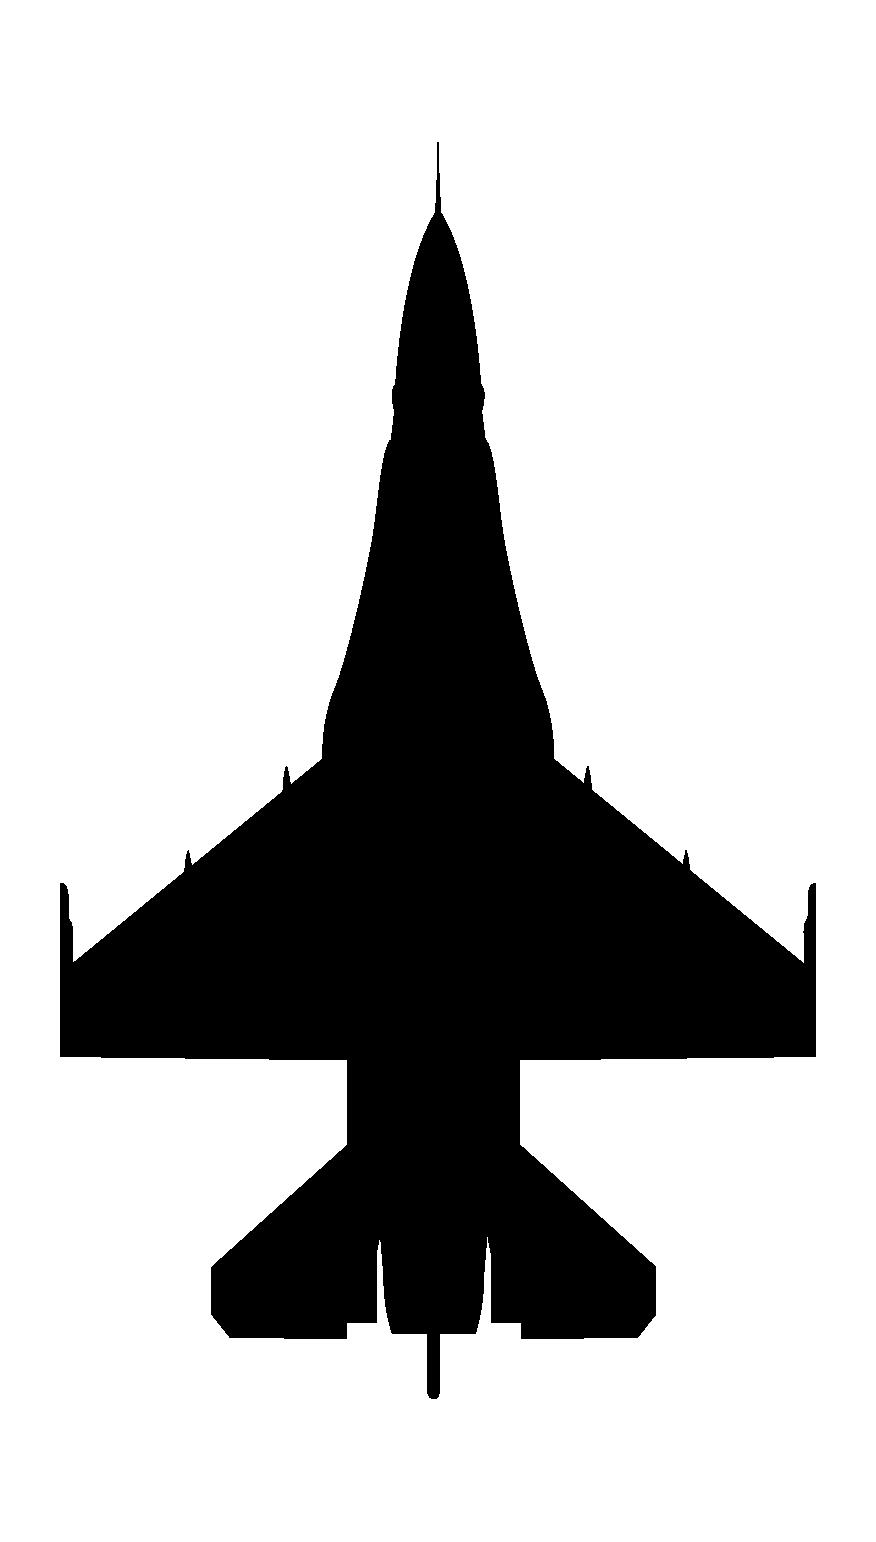
\includegraphics[
                    width=7.5mm,
                ]{diagrams/aircraft/silhouette_f16_top.pdf}
            };
            
            \node[yshift=-2mm] (wingfig) at (wing) {
                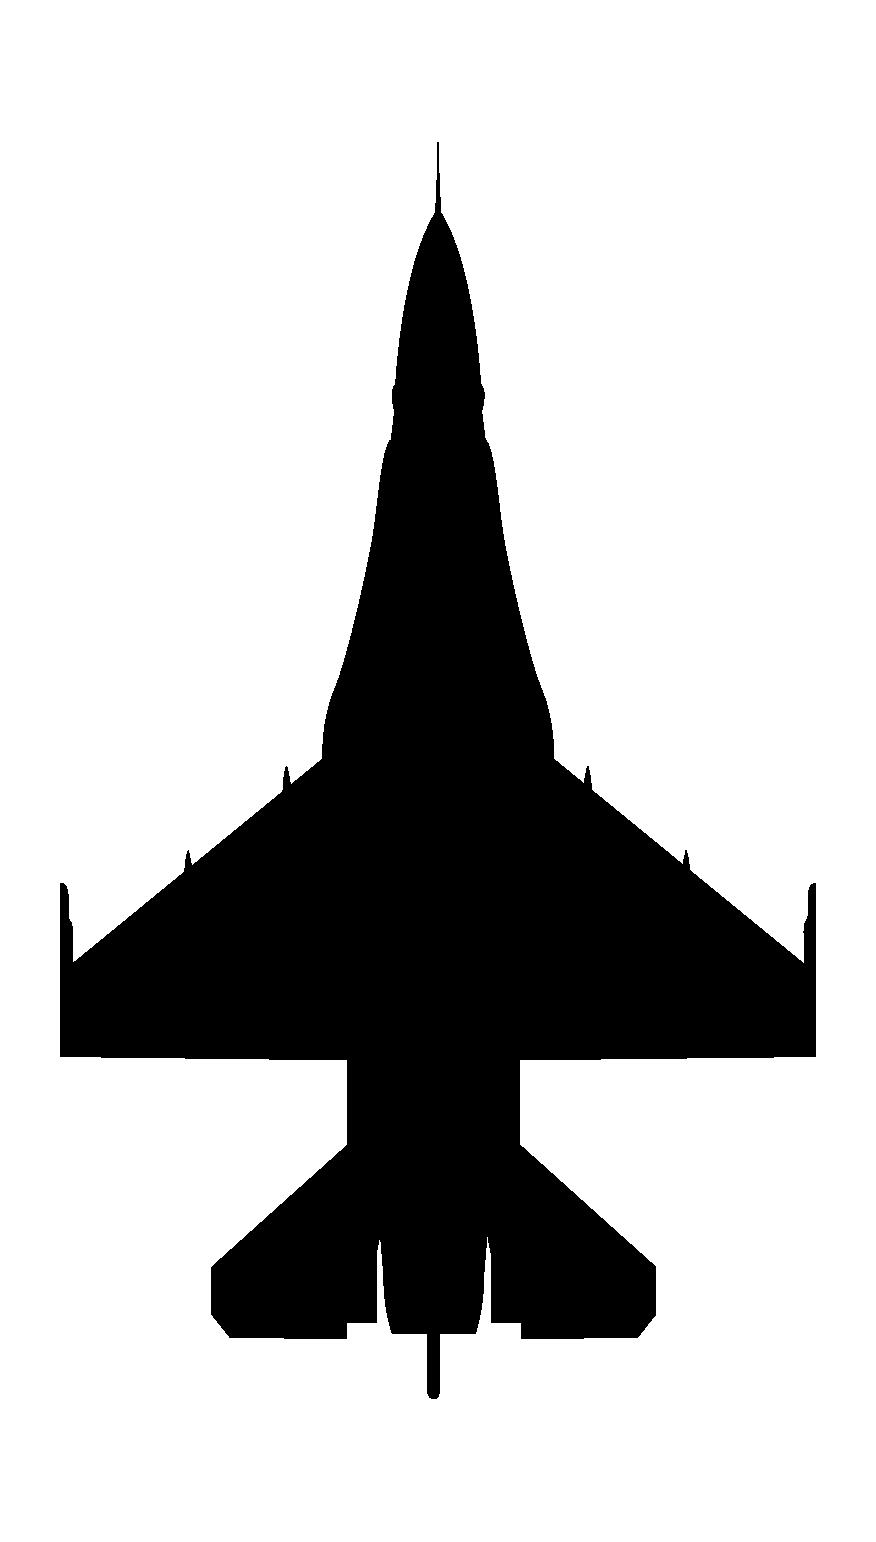
\includegraphics[
                    width=7.5mm,
                ]{diagrams/aircraft/silhouette_f16_top.pdf}
            };
    
            \draw[dotted]
            (lead) 
            -- node [font=\footnotesize] {4000'} ++(-30:35)
            node [font=\footnotesize, pos=1, right] {30 deg};
    
            \draw[dotted]
            (lead) 
            -- node [font=\footnotesize, below left] {5000'} ++(-60:35)
            node [font=\footnotesize, pos=1, right] {60 deg};
    
        \end{tikzpicture}
        \caption{wedge}
    \end{subfigure}

    \vspace{1em}
    \begin{subfigure}{0.65\linewidth}
        \centering
        \begin{tikzpicture}[auto, node distance=10mm, x=1mm, y=1mm, very thick, line cap=round,
            >={Latex[round]}
            ]
            
            \coordinate (lead) at (0,0);
            \coordinate (wing) at (15,-15);
    
            \node[yshift=-2mm] (leadfig) at (lead) {
                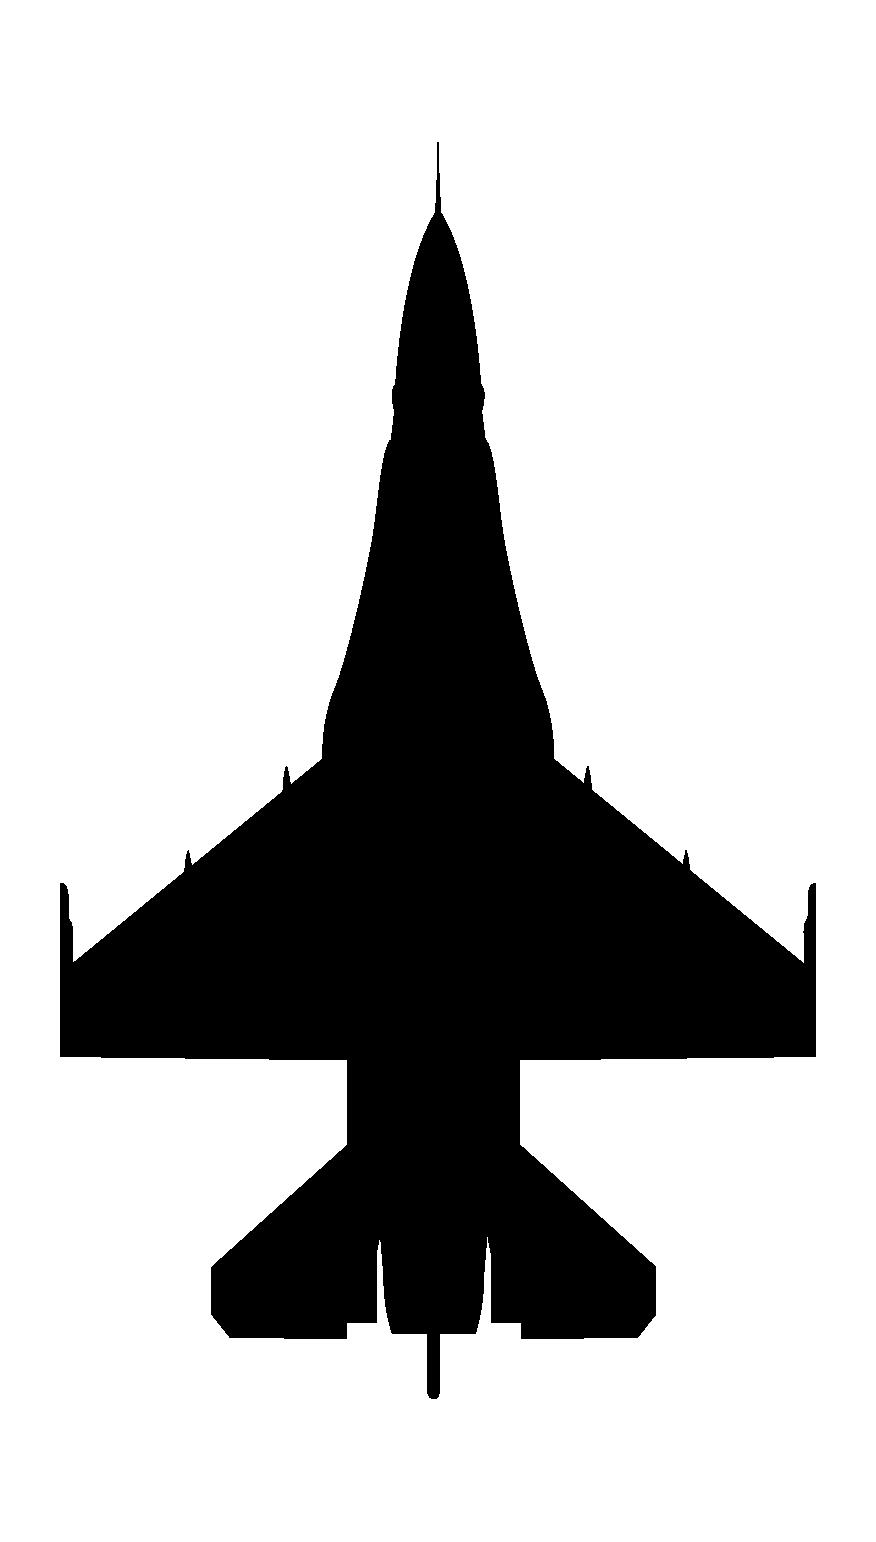
\includegraphics[
                    width=7.5mm,
                ]{diagrams/aircraft/silhouette_f16_top.pdf}
            };
            
            \node[yshift=-2mm] (wingfig) at (wing) {
                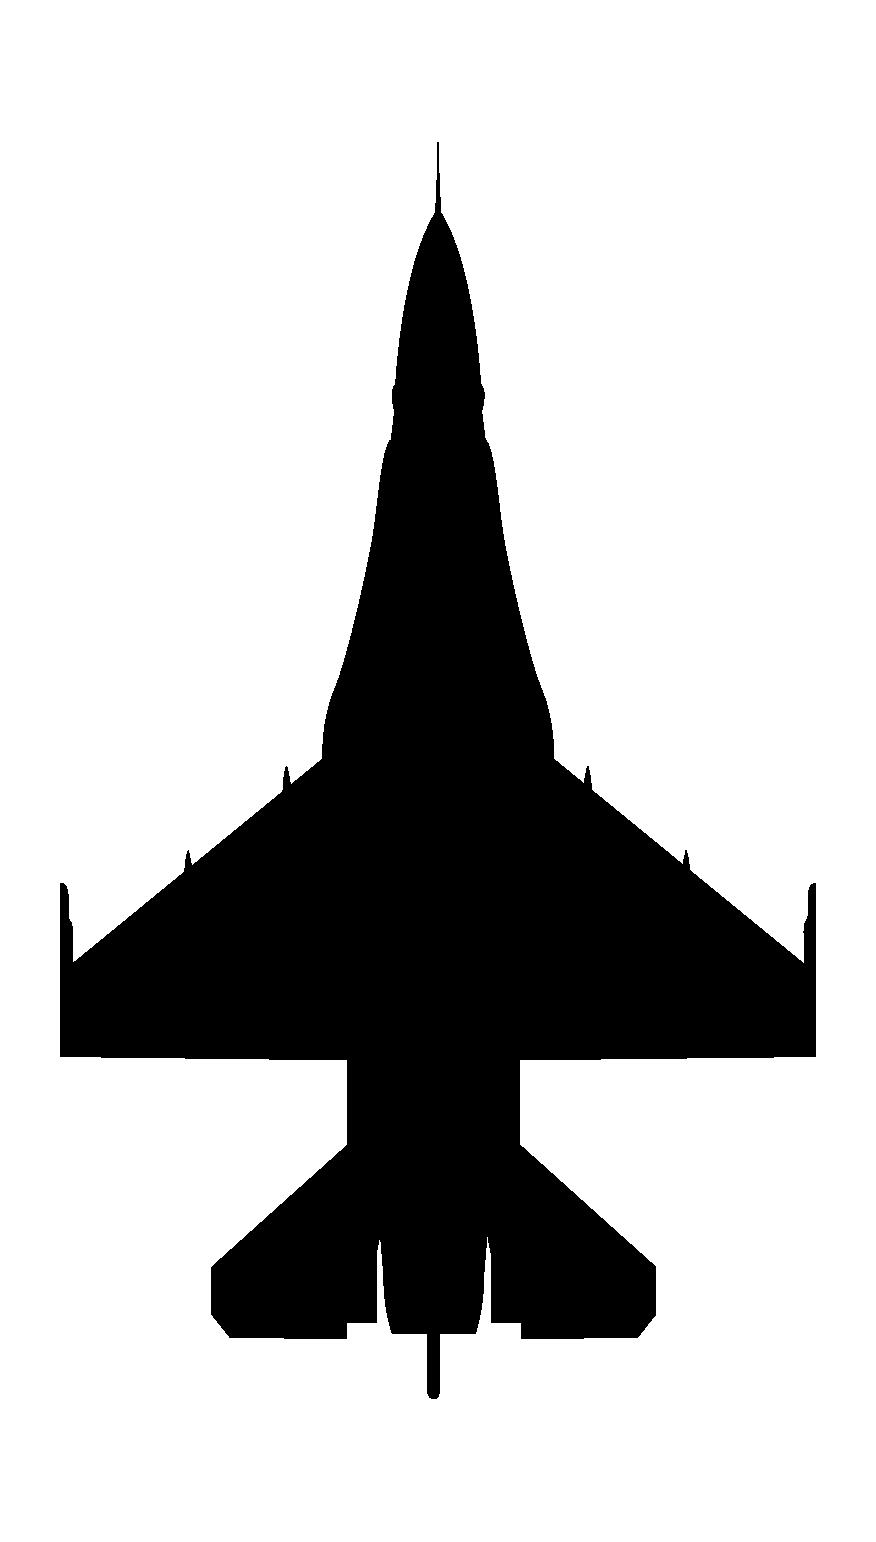
\includegraphics[
                    width=7.5mm,
                ]{diagrams/aircraft/silhouette_f16_top.pdf}
            };
    
            \node[
                draw, 
                ellipse, 
                minimum width=70mm,
                minimum height=10mm,
            ] (cone) at (0,-25) {};

    
            \node[
                draw, 
                ellipse, 
                fill=color1!20, 
                minimum width=18mm,
                minimum height=2mm,
            ] (inner) at (0,-25) {};

            \draw[dotted]
            (lead) 
            -- node [font=\footnotesize] {500'-3000'} (cone.east)
            node [font=\footnotesize, pos = 1, below right] {30 deg};
    
            \draw[dotted]
            (lead) -- (cone.west);
    
            \draw[dotted]
            (lead) -- (inner.east)
            node [font=\footnotesize, pos = 1, below right] {70 deg};
    
            \draw[dotted]
            (lead) -- (inner.west);

    
        \end{tikzpicture}
        \caption{fighting wing}
    \end{subfigure}
    \begin{subfigure}{0.3\linewidth}
        \centering
        \begin{tikzpicture}[auto, node distance=10mm, x=1mm, y=1mm, very thick, line cap=round,
            >={Latex[round]}
            ]
            \coordinate (lead) at (0,0);
            \coordinate (wing) at (12,-9.5);
    
            \node[yshift=-2mm] (leadfig) at (lead) {
                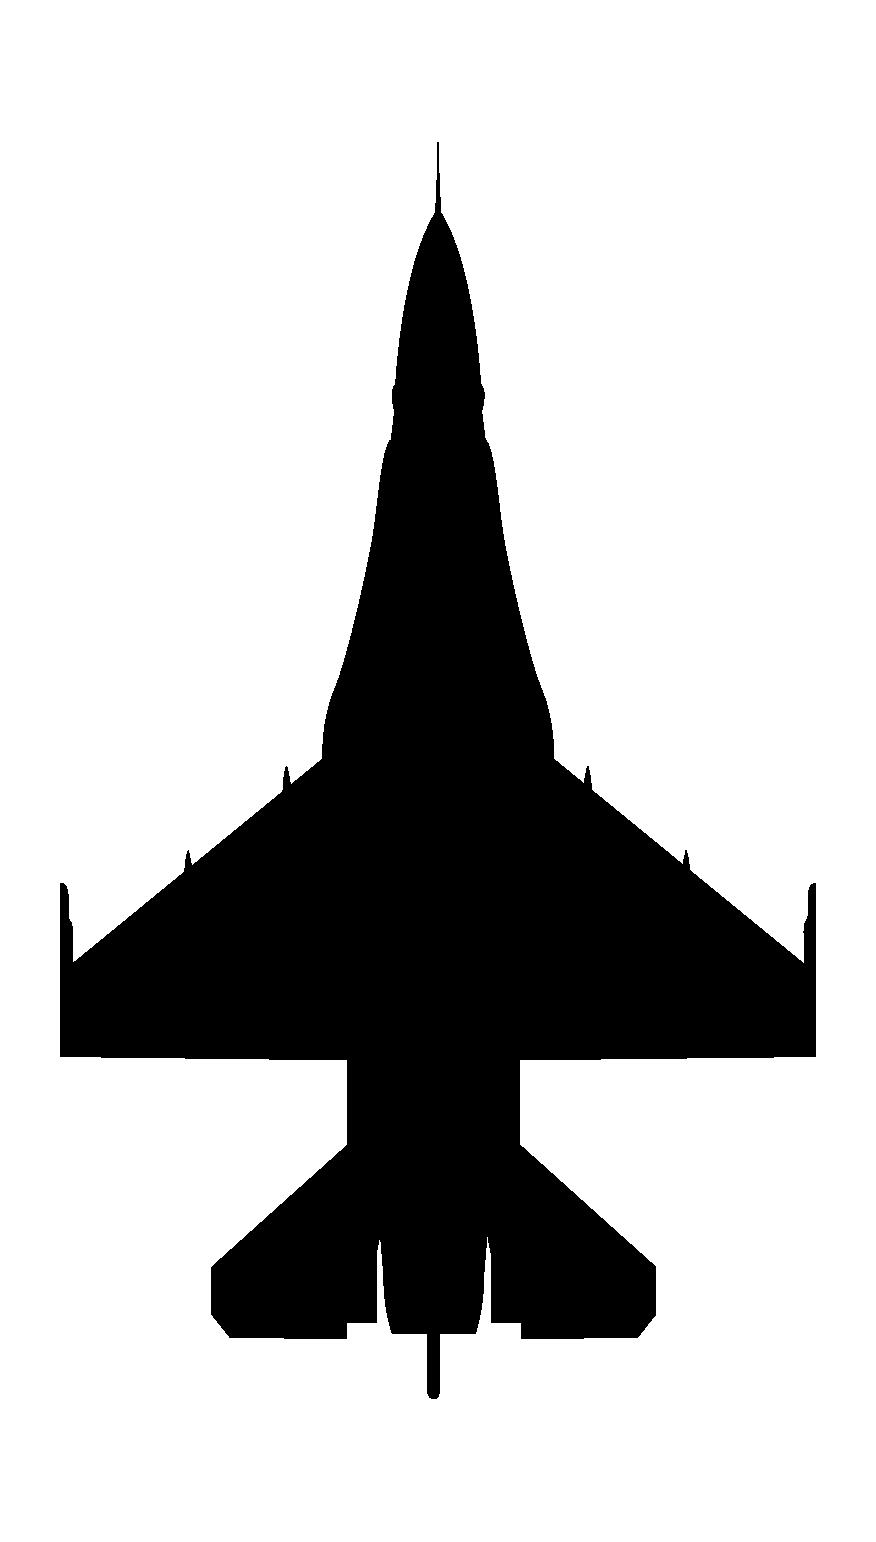
\includegraphics[
                    width=7.5mm,
                ]{diagrams/aircraft/silhouette_f16_top.pdf}
            };
            
            \node[yshift=-2mm] (wingfig) at (wing) {
                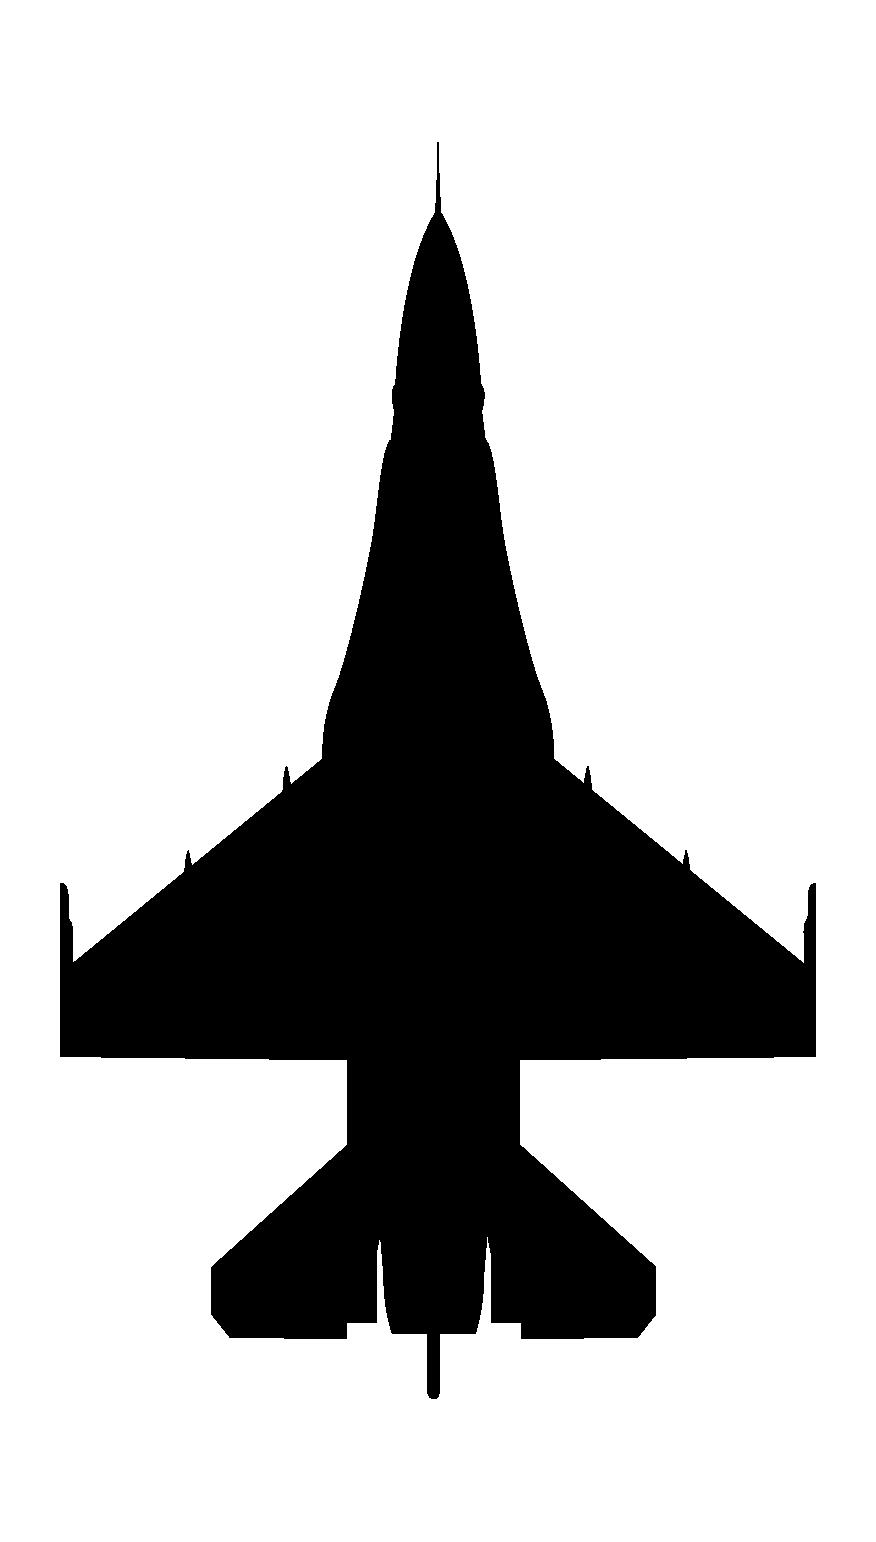
\includegraphics[
                    width=7.5mm,
                ]{diagrams/aircraft/silhouette_f16_top.pdf}
            };
    
            \draw[dotted]
            (lead) 
            -- node [font=\footnotesize] {66'} ++(-30:25)
            node [font=\footnotesize, pos=1, right] {30 deg};
    
            \draw[dotted]
            (lead) 
            -- node [font=\footnotesize, pos = 0.5, below left] {500'} ++(-40:25)
            node [font=\footnotesize, pos=1, below right] {40 deg};
    
        \end{tikzpicture}
        \caption{route / close}
    \end{subfigure}
    \caption{Two-ship formations}
\end{figure}

\cleardoublepage